\documentclass[
	%a4paper, % Use A4 paper size
	letterpaper, % Use US letter paper size
]{jdf}

\addbibresource{references.bib}

\author{Nan Xiao}
\email{nanx@gatech.edu}
\title{CS6750 HCI Summer 2021:\\Assignment M4}

\begin{document}
%\lsstyle

\maketitle

\begin{abstract}
	LinkedIn is one of the most popular social networks for professionals. Many of us rely on LinkedIn to expand connections and find new opportunities after graduation. In this project, we are going to study one task of LinkedIn - the searching function. The objective is to make a better interface design that the users can have a more relevant result on the LinkedIn search result page and accomplish the task.
\end{abstract}

\section{Qualitative Evaluation}
In this section, we will evaluate the Wizard of Oz prototype - using the voice signature to identify who you are talking with. Here is a quick recap of what the prototype looks like. As shown in Figure 1, when a user is talking to another person, the interface should be able to use the voice signature to identify the person's LinkedIn profile and make the suggestion to the user.
\begin{figure}[h]
	\centering
	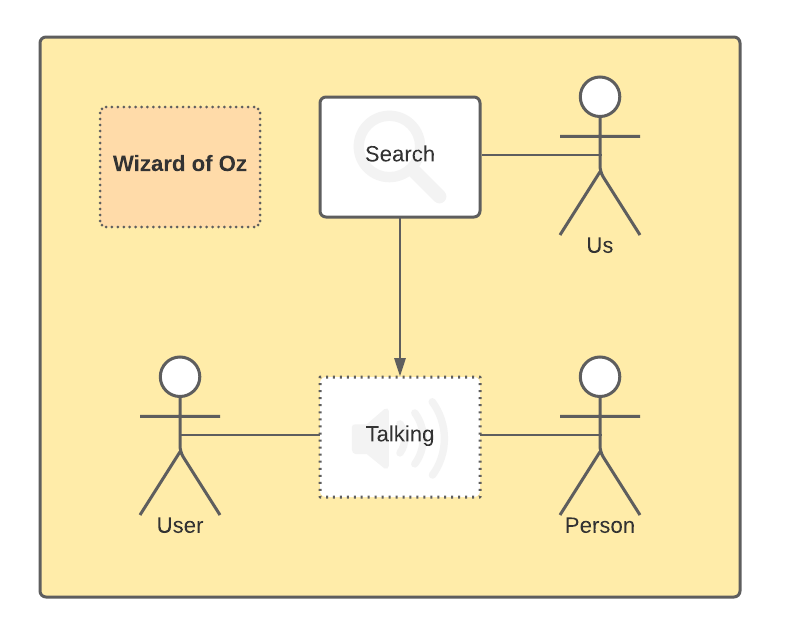
\includegraphics[height=5cm]{jdf-latex/Figures/Wizard of Oz.png}
	\caption{Wizard of Oz prototype for identify who you are talking to}
	\label{fig:wizard}
\end{figure}

\subsection{Evaluation Plan - Interview}
To perform the qualitative evaluation of the prototype, we will use the interview method. The participants are friends, family and classmates. They are chosen if they are regular LinkedIn users and in the age group both recent graduates and also seasoned professionals. Friends and family are easy to recruit. Classmates will be chosen from other OMSCS group projects. The interview will be conducted remotely except for families using Zoom or other tools. The response will be noted in the notepad for further aggregated analysis.

\subsection{Actual Content of Evaluation}
Because this is a new interface that people have no experience with before, we will provide a description of what the interface is capable of. The interview shall be conducted using semi-structured questions to allow interviewees to express concerns about the new interface.

\textbf{Interview Questions:}
\begin{enumerate}
    \item How often would you like to know the LinkedIn profile of the person you are talking with?
    \item How often do you forget your connections and spend much time searching people using different combinations of names and filters?
    \item How helpful would it be if you can search for someone without even knowing the name?
    \item What would you do if you want to know where your new colleague worked before?
    \item Would it be helpful if instead of you initiate the searching, the LinkedIn app can suggest the profile of the person you are talking with?
    \item What could be your concern if the LinkedIn search function can help you to identify who you are talking with?
    \item (If yes for the above question), do you think if you are allowed to turn off searchability of your own profile can help to mitigate the privacy concern?
    \item On which device would you prefer to see this function?
\end{enumerate}

\subsection{How the Evaluation will address requirements}
Refer to the \textbf{Table 1} of our requirements, our survey can help to identify gather data about functionality, usability and learnability. We will be able to understand whether the interface is easy to use, little time to understand, and able to accomplish their desired task.

Also, because we are semi-structured questions, the users can help to make suggestions about the existing interface. That will make the interface more user friendly and flatten the learning curve of a new user. Question about device compatibility is asked, but most likely the interface is more useful in the mobile device. 

\begin{table}[h] % [h] forces the table to be output where it is defined in the code (it suppresses floating)
	\caption{Requirements for the LinkedIn Search Function}
	\small % Reduce font size
	\centering % Centre the table
	\begin{tabular}{L{0.13\linewidth} L{0.13\linewidth} L{0.13\linewidth} L{0.13\linewidth} L{0.13\linewidth} L{0.13\linewidth}}
		\textbf{\-} & \textbf{Functionality} & \textbf{Usability} & \textbf{Learnability} & \textbf{Compatibility} & \textbf{Efficiency}\\
		\toprule[0.5pt]
		\textbf{Requirements} & User can find target in the search result & It is easy for the user to search & It takes little time for user to learn interface & The interface works on both mobile and website & The interface can also help expert user to accomplish task efficiently \\
		\midrule
		\textbf{Evaluation} & How many times user can find target in result & Interface is rated as easy to use for most users & How fast user start to use the interface & Users can accomplish task on both mobile and website & Users can finish task faster with shortcuts \\
	\end{tabular}
\end{table}

\section{Empirical Evaluation}
In this section, we will evaluate the text prototype - using predictive modelling to identify the most relevant result based on the search query and user profile. Here is a quick recap of what the prototype looks like. As shown in Figure 2, when a user clicks the search button, the interface should be able to use AI models to identify the most relevant LinkedIn profiles and rank the search results accordingly.
\begin{figure}[h]
	\centering
	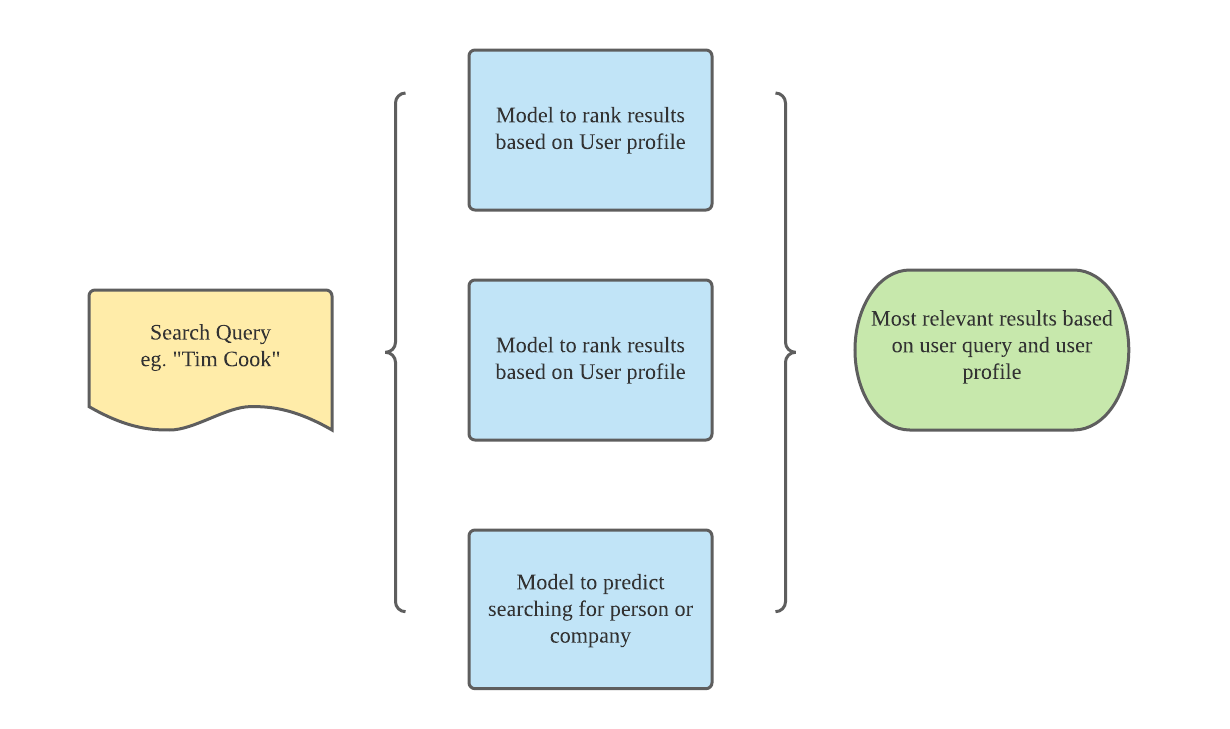
\includegraphics[height=5cm]{jdf-latex/Figures/Prototype.png}
	\caption{Use predictive modelling to give the most relevant search results}
	\label{fig:textprototype}
\end{figure}

\subsection{Define control and experimental conditions}
In this experiment, we will define our hypothesis as below:

\textbf{Null Hypothesis H0}: The new interface does not increase the CTR (Click-Through-Rate) in the search result page. It means the user is not more likely to find what he wants on the search result page.

\textbf{Alternative Hypothesis H1}: The new interface does increase the CTR (Click-Through-Rate) in the search result page. It means the user is more likely to find what he wants on the search result page.

\subsection{Experimental Method}

\begin{table}[h] % [h] forces the table to be output where it is defined in the code (it suppresses floating)
	\caption{Empirical Tests Selection}
	\small % Reduce font size
	\centering % Centre the table
	\begin{tabular}{L{0.2\linewidth} L{0.2\linewidth} L{0.2\linewidth} L{0.2\linewidth}}
		\textbf{IV} & \textbf{DV} & \textbf{Treatments} & \textbf{Recommended}\\
		\toprule[0.5pt]
		Categorical & Nominal & 2 or more & Chi-Squared test \\
		\midrule
		Categorical & Ordinal & 2 & KS test \\
		\midrule
		Categorical & Interval or Ratio & 2 & Student's t-test \\
		\midrule
		Categorical & Ordinal & 3 or more & Chi-Squared test \\
		\midrule
		Categorical & Interval or Ratio & 3 or more & ANOVA \\
		\midrule
		Categorical & Binomial & 1 or 2 & Binomial test \\
		\midrule
		Interval or Ratio & Interval or Ratio & 2 & Linear Regression \\
	\end{tabular}
\end{table}


We will use between-subjects analysis - the A/B testing method to verify if the alternative design is significantly better. Because our data is a ratio (CTR), based on Table 1, (\cite{joyner2016b}) it is better for us to use Student's Test method. Users are randomly selected into 2 groups (Group A and Group B), Group A will see the original interface, and Group B will see the new interface, which uses predictive modelling to better rank results. If we can see the final p-value < 0.05, that means we can successfully reject the null hypothesis and conclude that the new interface is significantly better at giving users better results.

\subsection{What lurking variables might confound the data}
According to Joyner (\cite{joyner2016c}), we have below tips to conduct a successful Empirical Evaluation.
\begin{enumerate}
    \item Control what you can, document what you can't
    \item Limit your variables
    \item Work backwards
    \item Script your analyses in advance
    \item Pay attention to power
\end{enumerate}

We may fail to control what a user may search for, maybe Group A users tend to make easier searches while Group B users tend to make more difficult searches. Then our conclusion may not be a fair comparison. Also, we may not recruit enough users that the sample size is not large enough to draw a conclusion. We should probably do a power analysis first to make sure the experiment satisfies the minimum sample size.

\section{Predictive Evaluation}
In this section, we will evaluate the wireframe prototype - using a photo to do facial recognition and match the LinkedIn profile. Here is a quick recap of what the prototype looks like. As shown in Figure 3, a user is able to upload a photo instead of searching for a name. The interface then should be able to use the facial recognition model to identify the most relevant LinkedIn profiles.
\begin{figure}[h]
	\centering
	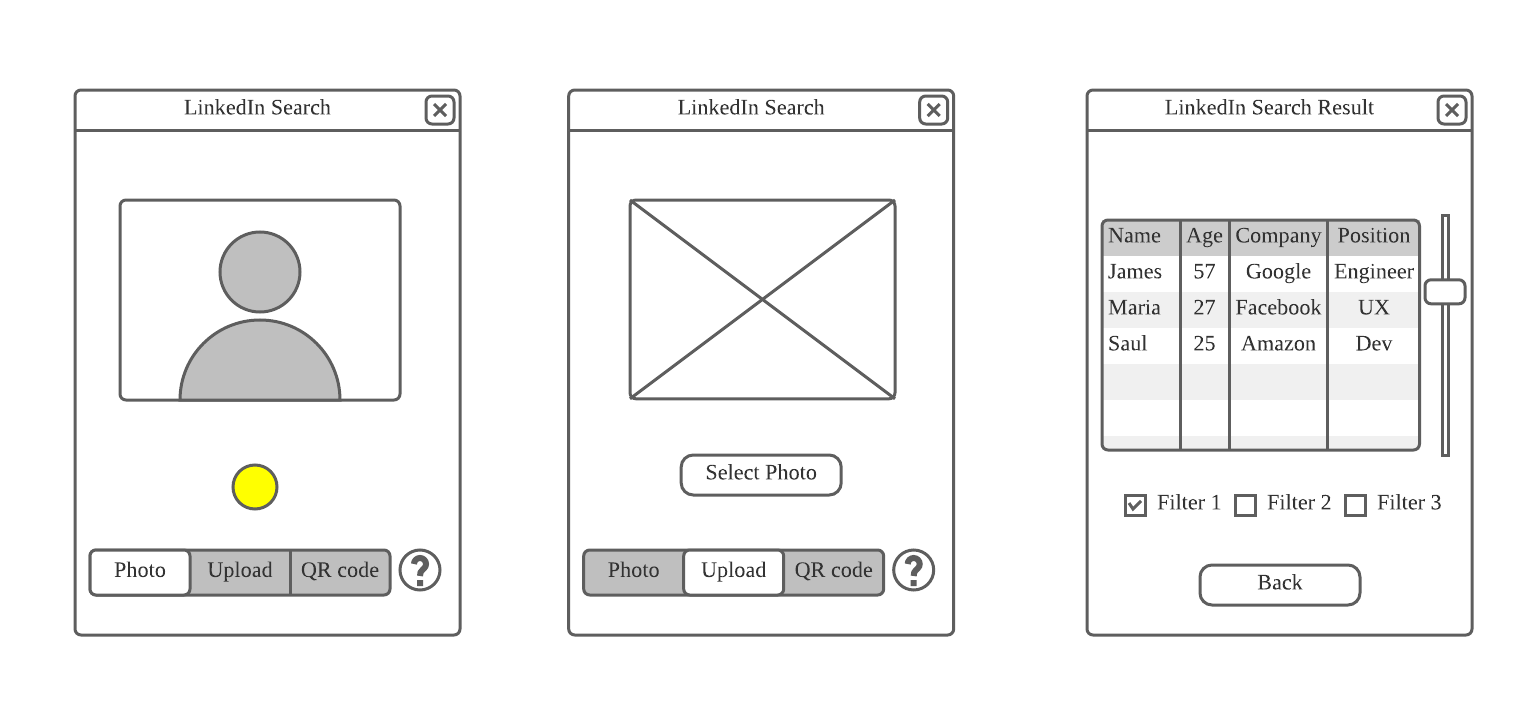
\includegraphics[height=5cm]{jdf-latex/Figures/LinkedIn Search Prototype.png}
	\caption{Wireframe of facial recognition in LinkedIn search function}
	\label{fig:wireframe}
\end{figure}

\subsection{Selecting Type of Task Analysis}
Because this is a new interface for the searching task, we would like to use \textbf{Cognitive Walkthrough} rather than the GOMS model. GOMS model is more suitable to evaluate an interface assuming the users are all expert users. By using the Cognitive Walkthrough, we can possibly identify the advantage of the new interface and potential cognitive barriers.

\subsection{Specific Tasks to be Addressed}

Cognitive task analysis adopts the predictor view of a human's role in the system. It generally follows below common sequence: (\cite{joyner2016d})

\begin{enumerate}
	\item Collecting preliminary knowledge
	\item Identify knowledge representations
	\item Apply focused knowledge elicitation methods
	\item Analyze and verify data acquired
	\item Format results for the intended application
\end{enumerate}

The \textbf{goal} of the user is to find the correct LinkedIn profile of the photo uploaded. It can be a single photo, a group of photos, or taking a real-time photo. The interface will be able to match that photo to the database and find the corresponding LinkedIn profiles of people in the photo. 

There are 3 \textbf{sub-tasks} for the user's top-level task (goal):
\begin{enumerate}
	\item Uploading the photo for searching the LinkedIn profile
	\item Taking a real-time photo for searching the LinkedIn profile
	\item Find the correct profile in the search result page
\end{enumerate}

The \textbf{operators} available in the interface:
\begin{enumerate}
	\item Clicking the LinkedIn search box
	\item Clicking the search by photo button
	\item Clicking Photo button
	\item Taking a photo using the built-in camera interface
	\item Clicking Upload button
	\item Clicking "Select Photo" button
	\item Uploading photo
	\item Scrolling through the search result page
	\item Selecting filters in the search result page
	\item Clicking profile in the search result page to redirect to the profile page
\end{enumerate}

\section{Preparing to Execute}
In this section, we will select 2 out of 3 evaluations from the last section to execute. According to Joyner, below are the advantages for different methods: (\cite{joyner2016a})

\begin{table}[h] % [h] forces the table to be output where it is defined in the code (it suppresses floating)
	\caption{Advantages for different evaluation methods}
	\small % Reduce font size
	\centering % Centre the table
	\begin{tabular}{L{0.5\linewidth} L{0.1\linewidth} L{0.1\linewidth} L{0.1\linewidth}}
		\textbf{Advantages} & \textbf{Qualitative} & \textbf{Empirical} & \textbf{Predictive}\\
		\toprule[0.5pt]
		Informs ongoing design decisions & Yes & - & Yes \\
		\midrule
		Investigates the participant's thought process & Yes & - & Yes \\
		\midrule
		Draws conclusions from actual participants & Yes & Yes & - \\
		\midrule
		Identifies provable advantages & - & Yes & - \\
		\midrule
		Provides generalizable conclusions & - & Yes & - \\
		\midrule
		Does not require any actual users & - & - & Yes \\
	\end{tabular}
\end{table}

We will choose Qualitative Evaluation (Interview) and Predictive Evaluation (Cognitive Walkthrough) for our execution. The reason is that it is difficult to conduct an Empirical Evaluation for our interface and collect enough data points to draw a conclusion. Especially, the interface requires an AI model in place for testing, that development is not feasible to deliver within time constraints.

\section{References}
\printbibliography[heading=none]


\end{document}